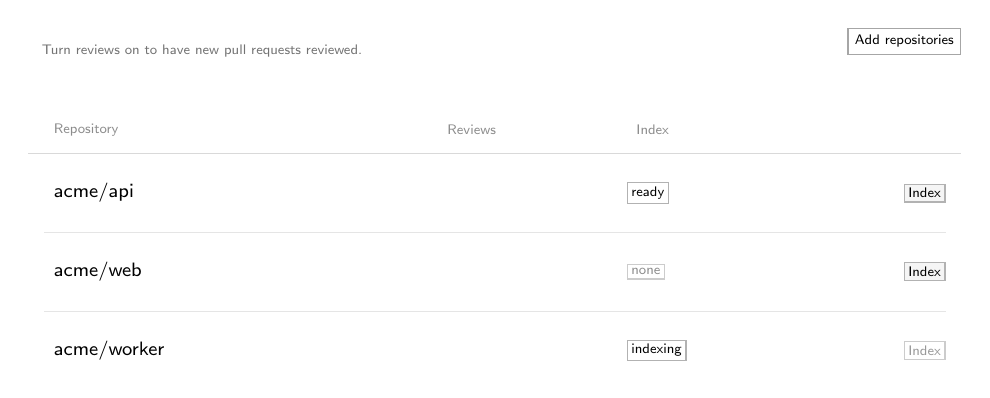
\begin{tikzpicture}[x=1cm,y=1cm]
  \wfchrome{Repositories}{7.25}

  \node[anchor=north west, font=\sffamily\tiny, text=black!55, text width=8.5cm] at (3.45,7.75)
    {Turn reviews on to have new pull requests reviewed.};
  \node[draw=black!35, fill=white, font=\sffamily\tiny, inner sep=2.5pt, anchor=north east] at (15.25,7.85)
    {Add repositories};

  \wfpanel{3.40}{3.20}{11.85}{3.75}
  \node[anchor=west, font=\sffamily\tiny, text=black!45] at (3.60,6.55) {Repository};
  \node[anchor=west, font=\sffamily\tiny, text=black!45] at (8.6,6.55) {Reviews};
  \node[anchor=west, font=\sffamily\tiny, text=black!45] at (11.0,6.55) {Index};
  \draw[black!15] (3.40,6.25) -- (15.25,6.25);

  \node[anchor=west, font=\sffamily\scriptsize] at (3.60,5.75) {acme/api};
  \wfon{8.7}{5.60}
  \node[anchor=west, font=\sffamily\tiny, draw=black!30, inner sep=1.5pt] at (11.0,5.75) {ready};
  \node[draw=black!30, fill=black!4, font=\sffamily\tiny, inner sep=1.5pt, anchor=east] at (15.05,5.75) {Index};

  \draw[black!10] (3.60,5.25) -- (15.05,5.25);
  \node[anchor=west, font=\sffamily\scriptsize] at (3.60,4.75) {acme/web};
  \wfoff{8.7}{4.60}
  \node[anchor=west, font=\sffamily\tiny, draw=black!20, text=black!45, inner sep=1.5pt] at (11.0,4.75) {none};
  \node[draw=black!30, fill=black!4, font=\sffamily\tiny, inner sep=1.5pt, anchor=east] at (15.05,4.75) {Index};

  \draw[black!10] (3.60,4.25) -- (15.05,4.25);
  \node[anchor=west, font=\sffamily\scriptsize] at (3.60,3.75) {acme/worker};
  \wfon{8.7}{3.60}
  \node[anchor=west, font=\sffamily\tiny, draw=black!30, inner sep=1.5pt] at (11.0,3.75) {indexing};
  \node[draw=black!20, text=black!40, font=\sffamily\tiny, inner sep=1.5pt, anchor=east] at (15.05,3.75) {Index};
\end{tikzpicture}
